\documentclass[a4paper,10pt,twocolumn]{article}
\usepackage[utf8]{inputenc}
\usepackage{fullpage}
\usepackage{amsmath}
\usepackage{amsfonts}
\usepackage{hyperref}
\usepackage{color}
\usepackage{graphicx}
\usepackage{soul}
\usepackage{xcolor}
\hypersetup{
    colorlinks,
    linkcolor={red!50!black},
    citecolor={blue!50!black},
    urlcolor={blue!80!black}
}
\newcommand{ \cbl}{\color{blue}}
\newcommand{ \cb}{\color{black}}
\usepackage[algoruled, vlined,linesnumbered]{algorithm2e}


\begin{document}

\title{Exploiting Object Symmetry for Efficient Grasping}
\author{
Can Erdogan $\;\;$ Ana Huaman $\;\;$ Heni ben Amor
}

\newcommand{\vech}[1]{\textbf{#1}}
\newcommand{\set}[1]{\textbf{#1}}

\maketitle

%% IDEAS
% - force map instead of collision map
% - invariance of height?
% - projection of fingers convex ?
% - add 3rd dimension (saturation)?
% - changing circle size by cutting through a cone. Allows for change in height.

%==================================================================================================
\begin{abstract}
In this, paper we introduce an efficient representation for robot grasping that exploits symmetry
properties of objects. The new representation forms a low-dimensional manifold, which can be used to
identify the set of feasible grasps during a sequential manipulation task. We analyse the properties
of this low-dimensional manifold and show that some of these properties can be used for fast
manipulation planning. We apply the introduced representation and planner to bi-manual manipulation
in humanoid robots.
\end{abstract}

%==================================================================================================
\section{Introduction}

Robots with advanced dexterous capabilities have the potential to revolutionize important
application domains such as healthcare, security, or manufacturing. Whether in structured
environments such as factories, or unstructured environments such as homes, grasping is often the
first step in the physical interaction between a robot and its surroundings. The generation of
grasps on objects is therefore at the heart of plan generation for physical tasks. However, to date most grasp
planning methods are mainly focused on generating physically stable grasps without incorporating
immediate or future task constraints. 

Many well established algorithms assume only a single action and do not include foresight and
reasoning about next actions. However, when picking up a mug, it is important to select a grasp that
facilitates the next action to be performed. For example, in case the next action is a pouring motion, the robot
needs avoid grasps that would cover the rim of the object. In contrast, if any of the next actions
involves placing the mug on the table, the robot cannot choose any grasp in which fingers touch the
mug's base. 


\begin{figure}[t]
  \begin{center}
    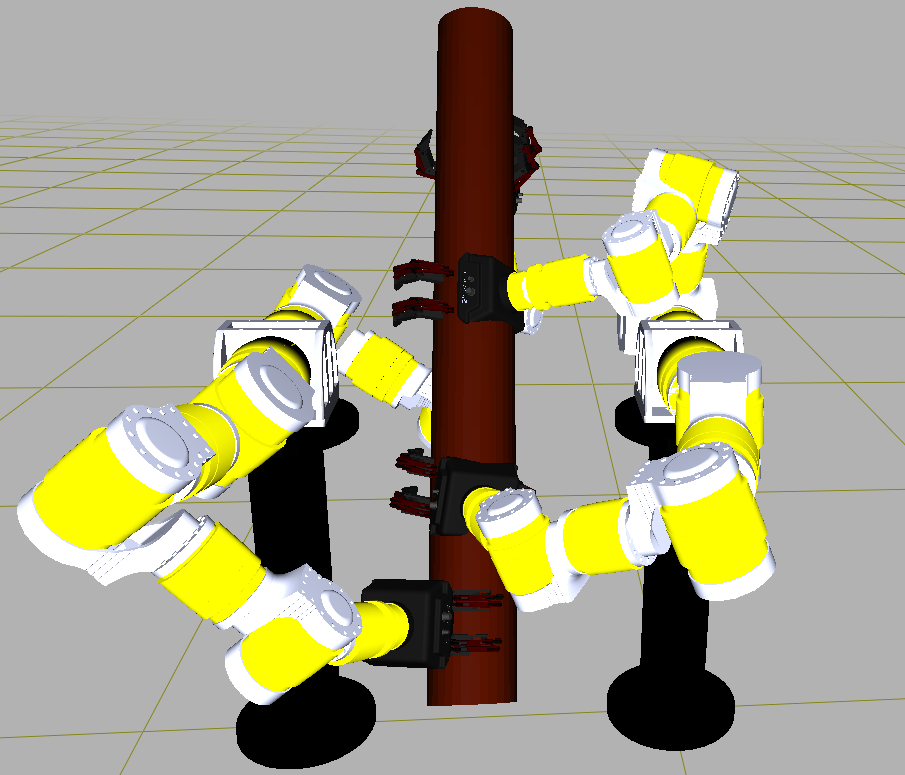
\includegraphics[width=1.0\linewidth]{./images/showOff.png} \quad 
  \end{center}
  \caption{The manipulation of a heavy wooden log by two robots, planning for a pair of bimanual grasps}
  \label{fig:showOff}
\end{figure}


Many grasp representations are based on a floating hand, thereby representing only the
end-effector and ignoring the embodiment of the entire robot in environment. As a result, infeasible
grasps are generated and have to be pruned out in a post-processing step. This can be particularly
limiting in bi-manual, sequential, and co-worker scenarios, in which the actions of one agent are likely to violate the constraints of another agent. In these scenarios, grasps need to be carefully chosen, such that they do not violate constraints imposed by a second arm, a human interaction partner, or a future action. 

In this paper, we address the issue of manipulation planning with task constraints. We are
particularly interested in tasks that involve several subtasks or several interacting agents.
Planning grasps for such tasks can rapidly become computationally infeasible due to the large search
space. The key insight of this paper is that re-occurring patterns in the geometry of shapes can be
exploited to drastically reduce the space of solutions. We will introduce a low-dimensional,
object-centered representation for grasp planning which is based on rotational symmetries. The
symmetric nature of the objects allows us to update our representation as the object is rotated around
the axis of symmetry. \emph{Since the object is symmetric any stable grasp can be rotated around the
axis yielding a family of feasible grasps}. We will show that this basic property leads to a
significant reduction of the search complexity in grasp planning. Specifically, this property allows us
to generate multiple grasps around the object which is useful for bi-manual tasks and cooperative
robot hand over tasks. Figure 1 demonstrates an example where a rotationally symmetric log is manipulated by two robots using both arms. In addition, it allows us to identify a single grasp that is useful for a
sequence of tasks.



%
%	
%
%\item Advantages of approach?
%	\begin{enumerate}
%	\item 
%	
%\item Contributions?
%	\begin{enumerate}
%	\item new representation for efficient parameterization of stable grasps 	
%	\item discussion of properties of representation induced by symmetric objects
%	\item a grasp planning algorithms using representation to achieve sequential and 
%		  bimanual tasks  
%	\end{enumerate}
%	\end{enumerate}
%	
%	
%
%\begin{enumerate}
%\item What is paper about?
%	\begin{enumerate}
%	\item Robots are required for assisting in collaborative tasks
%	\item Especially physical taks, e.g., domestic environments, healthcare, 
%		  defense, manufacturing 
%	\item Robots need manipulation and grasping capabilities (one of most 
%		  important behaviors)
%	\item Grasping is at the heart of planning physical tasks 
%	\end{enumerate}
%
%\item What is the problem?
%	\begin{enumerate}
%	\item Grasp planning taking into account environment and task constraints
%	\item Current grasp representations are based on a floating hand, which only 					  represents the end-effector and ignores embodiment of whole robot in
%		  environment. As a result, infeasible grasps are generated and have to be
%		  pruned out in a post-processing step. 
%	\item Well established algorithms assume only one action, and do not include
%		  foresight and reasoning about next actions to perform. Example, pouring
%		  into a cup. Example, putting mug into washing machine.
%	\item Motion planning with multiple subtasks -> planning needs to be fast 
%		  as possible (complexity)
%	\item !Try to show that separation of planning and grasp selection is naive
%	\item Especially in bi-manual, sequential and co-worker scenarios, complexity increases
%	\end{enumerate}
%	
%\item What is our approach?
%	\begin{enumerate}
%	\item Reoccurring patterns in the geometry of shapes can be exploited
%	\item Rotational and linear symmetries and extrusions can be exploited
%	\item In this paper we focus on rotational symmetries
%	
%	\item Object-centered representation
%	\item Project world and hand information into the representation, thereby taking
%		  into account reachability and collisions
%	\item Examples, picture of symm. object with two hands and hands are projected 
%		  into manifold.
%	\item 
%\end{enumerate}
%==================================================================================================

\section{Related Work}
Robot grasping is a heavily studied sub-field of robotics.
Until recently, most approaches have focused on the problem 
of generating stable grasps on objects. Given a model of an object, a hand shape is synthesized 
that allows the physically stable manipulation of the object~\cite{Klank2009, Kragic2001}.
A prevalent approach is to modify the grasp parameters 
until a hand shape is found which is optimal w.r.t.~a given criterion, such as force closure \cite{nguyen}, or grasp wrench space \cite{Borst}. For recent surveys 
of the grasp synthesis literature the reader is referred to \cite{Bohg2014} and \cite{Sahbani2012}.

To efficiently synthesize a 
variety of grasps, objects are often modelled
using primitives, such as bounding boxes \cite{huebner2008selection}, medial axis
representations \cite{przybylski2010unions}, superquadrics \cite{goldfeder2007grasp}, 
or simple geometrical shapes including cylinders, boxes and spheres \cite{miller2003automatic}.
Another way of increasing efficiency is by reducing the dimensionality of
the space of possible hand configurations. In \cite{ciocarlie2009} and \cite{benamor}, 
dimensionality reduction techniques are used to project the space of
hand shapes onto a low-dimensional manifold of two to three dimensions.
However, in the above approaches, reachability and possible collisions
during motion execution are only analyzed in a post-processing step after 
grasps are generated. Hence, possibly unreachable or unsafe grasp configurations 
are produced. Recent approaches have tried to bridge the divide through simultaneous 
grasp synthesis and motion planning~\cite{Vahrenkamp12d}. Still, as noted in \cite{dang}, 
looking solely at the stability of the grasp, or other
immediate criteria ignores task constraints which 
are induced by the subsequent manipulations of the object. 
A grasp is often highly dependent on the task 
to be performed and should be chosen with next actions in mind.

Dang et al. \cite{dang} incorporate task constraints by 
semantically annotating grasps from a database. These grasps
are then mapped onto a new object using local optimization.
While this approach is a substantial step towards task-based
grasp synthesis, it still requires prior human annotations of 
a grasp dataset. In a similar vein, Antanas et al. \cite{antanas} 
use a probabilistic logic module to semantically reason
about pre-grasp configurations with respect to the intended tasks.
By exploiting symbolic world knowledge stored in object/task ontologies,
they can infer appropriate grasps for a given task. 
A machine learning approach with a similar goal
was introduced by Song et al. \cite{song}. Their approach 
uses a Bayesian Network to learn task constraints for 
object manipulation. 

The need for sufficient \emph{foresight} 
during action selection has recently been discussed in the hierarchical
planning literature~\cite{LevihnIROS13}. Levihn and colleagues
argue that look-ahead into future plans is important to 
avoid making short-sighted choices. While close in spirit to the 
work presented in our paper, the work of Levihn and colleagues 
concentrates on the task of moving among obstacles and does not 
include grasp synthesis.

In this paper, we show how inherent shape properties, specifically
rotational symmetries, can be used to efficiently generate 
task-constrained grasps. Object symmetries have long
been studied in the computer vision literature.
Recently, various studies have indicated that symmetries 
can be exploited for grasping~\cite{kroemerHumanoids2012, bohg2011mind}. However, 
these studies have mostly focused on how to generate complete 
meshes from partial point clouds.

%==================================================================================================

\section{Manifold Representations for Rotationally Symmetric Objects}

Projecting manipulation constraints such as collisions with the environment and robot
manipulator limitations (e.g. reachability) onto object surfaces can facilitate the search
for feasible grasps. In this work, we demonstrate that particularly for rotationally
symmetric objects, which do not have any surface protrusions or cavities, a number of grasping sub-problems
such as finger placements, wrist pose, and collision-free inverse kinematics are simplified. 
Inspired by the texture mapping literature in computer graphics, we begin with the two-dimensional manifold
representation of rotationally symmetric objects whose surfaces can be unwrapped
into simple planes. The goal is to use this low-dimensional representation to accumulate
multiple task constraints in the same local object space and then, efficiently identify 
grasps that satisfy all the future actions. 

%==================================================================================================
\subsection{Cylindrical Surface Parametrization}

Coordinate spaces characterized by rotations around an axis can be parametrized by cylindrical
parameters where a vector $\vech{z}$ represents the principal orientation and the polar axis
$\vech{a}$ captures the secondary direction in the reference plane perpendicular to $\vech{z}$. 
Using their intersection $\vech{o}$ as the origin, any point in the Euclidean coordinate system can
be represented in this coordinate system by computing the projection of the point onto the
$\vech{z}$ axis, its distance to the axis, and the angle between the polar axis $\vech{a}$ and its
projection onto the reference plane. 

Figure \ref{fig:representation} demonstrates the representation
of a point on a rotationally symmetric object in terms of the parameters $[h, r, \theta]^T$
that correspond to the height along $\vech{z}$, the radius $r$ of the circle parallel to the
reference plane that includes the point, and the angle $\theta$ between $\vech{a}$ and the point
projection onto the reference plan. Note that the reference plane is arbitrarily placed 
on the bottom surface of the object and the polar axis can be freely chosen within this plane. 

\begin{figure}[t]
  \begin{center}
    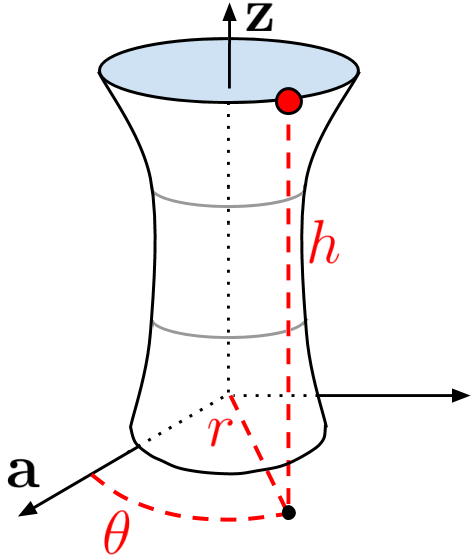
\includegraphics[width=0.5\linewidth]{./images/representation.png} \quad 
  \end{center}
  \caption{Cylindrical coordinate system to parameterize points on a rotationally symmetric object}
%   \caption{A of a
%   rotationally symmetric object. The axis $\vech{a}$ corresponds to the polar axis, while $\vech{h}$
%   is the axis of symmetry. Any point on the surface can be represented using height $h$, radius $r$,
%   and angle $\theta$. }
  \label{fig:representation}
\end{figure}

A significant observation about the representation of rotationally symmetric objects in cylindrical
coordinates is the dependency between the radius $r$ and the height $h$ parameters. For a given shape $S$,
all the points on $S$, at some height $h$ along the principal axis $\vech{z}$, have the same distance
$r$ to the axis: $\forall \vech{p} \in S$ s.t. $\vech{p} \cdot \vech{z} = h$, $dist(\vech{p}, \vech{z}) = r_S(h)$. The
function $r_S(h)$ represents the inherent curvature of the shape - for instance, for a cylinder, $r
= c$ for some constant $c$. Based on this observation, we can conclude that any contact point $\vech{p}$ on
an object shape $S$ can in fact be parameterized minimally by two variables, $h$ and $\theta$.
In this work, we show that analyzing the task constraints, robot limitations and contact models 
in this low-dimensional subspace leads to significant efficiency gains in grasp planning.

%==================================================================================================
\subsubsection{Mapping Euclidean Coordinates to a Cylindrical Coordinate System}

To reason about tasks traditionally expressed in Euclidean coordinates, we introduce a mapping 
between the representation of a point in the Euclidean world frame, $p_w$, to the $\vech{x} = [h,\theta]^T$
parameters in the a cylindrical coordinate system $\mathbb{S}$. First, we define the local object frame $L$ in the
Euclidean coordinate frames by using the principal axis (i.e. axis of symmetry) $\vech{z}$, the polar axis $\vech{a}$, and
their cross-product. Given the pose of an object in the world coordinates, $T^w_l$, we can first
transform the point into the local object space, $p^l = T^l_w ~ p^w$, and then map it to the surface
representation $\vech{x}$ using the function $f: \mathbb{R}^3 \rightarrow \mathbb{S}$: 
% TODO Add [h \theta] to this equation?
\begin{equation}
  f(\vech{p}^l) = f([x,y,z]^T) = \left[ \begin{array}{c} z \\ atan2(y,x) \end{array}\right].
\end{equation}
Once a planner reasons about the environment and a contact point is determined in the cylindrical surface representation,
we need to map it back to the Euclidean space using an inverse mapping $f^{-1}: \mathbb{S} \rightarrow \mathbb{R}^3 $:
\begin{equation}
  f^{-1}(\vech{x}) = f^{-1}([h, \theta]^T) = \left[ 
  \begin{array}{c}
  r(h) ~ cos(\theta) \\ r(h) ~ sin(\theta)\\ h 
  \end{array} \right]. 
\end{equation}
Fig.~\ref{fig:unfolding} depicts the forward mapping process moving from the local object frame to the cylindrical surface representation. Observe that the surface of the example soda can be unwrapped into a smooth finite two-dimensional plane with minimal distortion because the object is rotationally
symmetric, and does not have protrusions nor cavities. 
\begin{figure}[t!]
  \begin{center}
    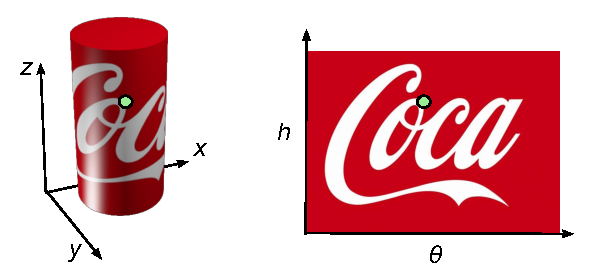
\includegraphics[width=0.45\textwidth]{./images/unfolding.pdf} \quad
  \end{center}
  \caption{The points on the 3D surface (left) are projected onto a 2D cylindrical manifold.}
  \label{fig:unfolding} 
\end{figure}

%==================================================================================================
\subsection{Grasp Manifold}

\textit{Stable grasps can be rotated around the principle axis of rotationally symmetric objects
without having to modify the hand shape}. Moreover, the relative rotation between a predefined grasp
and an object can be captured with a simple linear motion model in the reduced 2D cylindrical
manifold. To demonstrate the advantages of this key idea, we begin our analysis with a simplified
manipulation model where a point on the object surface corresponds to a wrist position during
grasping. Moreover, the hand is assumed to be parallel to the base of the object such that the plane
between the grasping fingers is perpendicular to the axis of symmetry. 

Given a predefined hand shape and a task definition, the planner needs to choose a contact point,
$\vech{x} = [h, \theta]$, that represents its wrist position. Feasible contact points are characterized
by collision-free inverse kinematic solutions where at least one manipulator pose should exist that both reaches the desired point and does not collide with the environment. Fig.~\ref{fig:bottlemapping} visualizes this concept. We can discretize the manifold representation using a regular grid. Each cell can then be mapped to the bottle object. For each cell of the
discretized manifold, using the center point  as the reference for the wrist, we attempt to compute a collision-free inverse kinematics solution. In Fig.~\ref{fig:bottlemapping}, red cells indicate collisions, while green cells indicate collision-free grasp locations. 

\begin{figure}[t]
  \begin{center}
    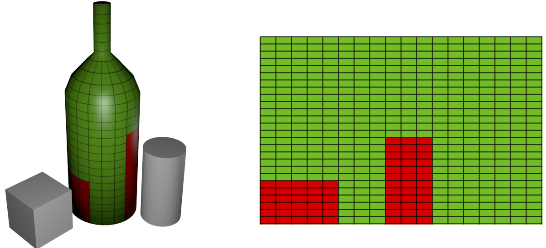
\includegraphics[width=0.45\textwidth]{./images/bottlemapping.png} \quad
  \end{center}
  \caption{For each cell of the wine bottle we check for collisions and reachability and store the result in a map representing the corresponding low-dimensional manifold. Red cells are grasp locations that would lead to collisions or are unreachable.}
  \label{fig:bottlemapping} 
\end{figure}
In addition to the physical feasibility of a contact point, its functionality towards accomplishing tasks also needs to be taken into account in grasp selection. For instance, if an object is picked with the purpose of
placing it down in another cluttered environment, collisions in the second scene also need to be accounted for. Similarly, a task may require an object to be configured at a specific pose, i.e. pouring water from a bottle to a cup, in which case the planner should account for the reachability of
that pose with the \textit{foresight} that the same grasp would have to be utilized. 

%==================================================================================================
\subsubsection{Modeling Task Constraints in Cylindrical Space}

Most everyday grasps require reasoning about multiple tasks even though the tasks may take place in substantially different environments with varying constraints on the pose of the manipulated
object. Although the locations and requirements of the tasks may vary, they all impose constraints 
on the same gripper-object system since once an object is picked, the grasp cannot be changed. 
We exploit the \textit{invariance} of the gripper-object relationship in manipulation tasks with 
rotationally symmetric objects, where the task descriptions naturally account for all the degrees 
of freedom but the rotation around axis of symmetry since the rotation does not effect object properties. The goal is to autonomously exploit the under-constrained task specifications by planning for object rotations and grasp positions. 
\begin{figure*}[ht]
  \begin{center}
    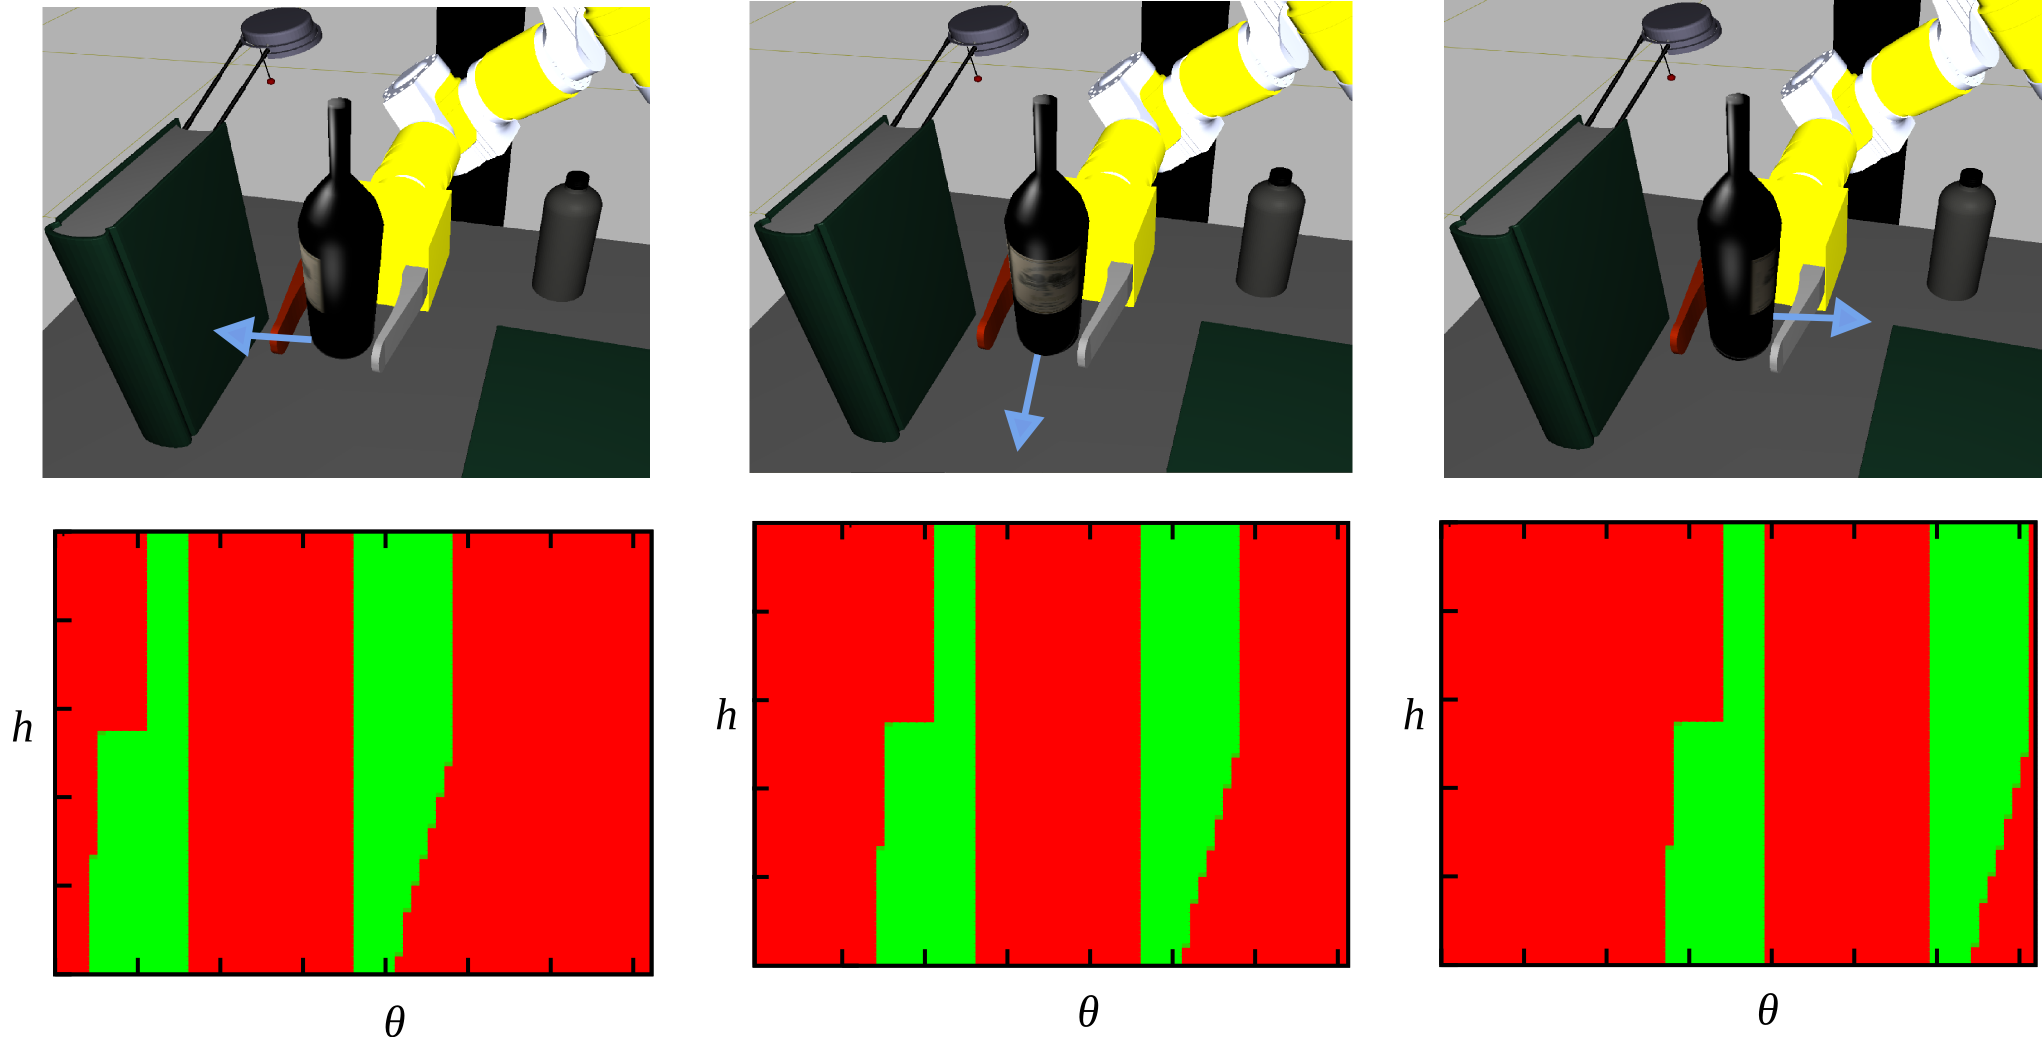
\includegraphics[width=0.75\linewidth]{./images/rotatingWine.png} \quad
  \end{center}
   \caption{Visualization of the task constraints with a rotating bottle. We can see that the entries of the low-dimensional manifold only shift when the object rotates around its axis of symmetry. This feature is a key insight of this paper. It follows, that there is a simple update procedure for the entries.}
  \label{fig:rotatingwine} 
\end{figure*}
By only modelling grasps that are perpendicular to the axis of symmetry, e.g. grasp rotates around object, we induce a coupling between gripper and object poses. Now, \textit{given a single pair of gripper and object poses that is known to satisfy task constraints, an infinite number of new pairs can be generated by rotating the gripper around the object by some $\theta$ degrees and rotating the object around itself by $-\theta$}. Moreover, by determining the feasible set of contacts for an initial object
pose which satisfies task requirements, we can extrapolate to a family of object rotations and corresponding contact placements. This extrapolation is only feasible because the rotation of the object around its axis and the rotation of the grasp around the object are coupled by the $\theta$ variable around the principle axis $\vech{z}$ and thus, we reason about task
constraints in the cylindrical parameter space.

A crucial property of this representation is that the produced map can
be efficiently updated when the object is rotated around its axis of symmetry. More specifically, a rotation around the z-axis corresponds to a shift along the $\theta$ dimension. 

%==================================================================================================
%\newpage
\subsubsection{Extrapolating Task Constraints to new Object Rotations}
The analysis of grasp feasibility for a given object pose and task description can be utilized to reason
about grasp selection if the object is rotated only around its axis of symmetry. The idea is that the 
coupling between the rotation of the grasp around the object pose and the rotation of the object around
its own principle axis can be utilized to generate previously examined grasps for new object rotations
and to adopt the successful examples. The invariance of task constraint effects on gripper-object
systems to interactions between the gripper and the object poses that do not change gripper configuration
in the task space can be analyzed formally. 

Let the function $m: \mathbb{S}, SE(3) \rightarrow \{0,1\}$ represent a mapping from a 6-DOF object pose $T^w \in SE(3)$ and a contact pose on the object surface, $\vech{x} = [h, \theta]^T \in \mathbb{S}$, to a binary evaluation of whether a grasp is feasible. The feasibility of a grasp may depend on a variety
of criteria such as inverse kinematics, collisions, torque limits, manipulability and etc. In this work,
we focus on collision-free inverse kinematics and define the operator $ik: SO(3), \mathbb{R}^3 \rightarrow \{0,1\}$
that evaluates whether an arm configuration exists that can achieve the end-effector rotation $R^w_e \in SO(3)$ and location $t^w_e \in \mathbb{R}^3$. 

We claim that given the mapping of feasibility grasps for an initial object pose $T^w_o$, the feasibility of any 
grasp $x \in \mathbb{S}$, for a new pose $T^w_{o_2}$, can be deduced by using the previous mapping:

\begin{equation}
  m([h,\theta],T^w_{o_2}) = m([h,\theta+\delta], T^w_o)
\end{equation}

\noindent where $T^w_{o_2} = T^w_o R^z(\delta)$ where $R^z(\delta)$ is a rotation matrix around the
local $z-axis$ by angle $\delta$ (the notation $T^z(\delta)$ also represents a
transformation matrix with the rotation $R^z(\delta)$ but no translation). The claim is proven
by showing that the gripper and object rotations counteract each other:

\begin{alignat}{2}
  m(&[h,\theta]^T,T^w_{o_2}) 	=	\notag \\
				&= ik(R^w_{o_2} R^z(\theta), 			&&T^w_{o_2} f^{-1}([h,\theta]^T)) \\
				&= ik(R^w_o R^z(\delta) R^z(\theta), 		~&&T^w_{o_2} T^z(-\delta) f^{-1}([h,\theta+\delta]^T)) \label{eq:proof_key} \\
				&= ik(R^w_o R^z(\theta+\delta), 		&&T^w_o f^{-1}([h,\theta+\delta]^T)) \\
				&= m([h,\theta+\delta]^T, T^w_o). 				
\end{alignat}

The proof starts by reducing the mapping to the inverse kinematics problem where the wrist orientation is computed
in the world coordinate frame by composing the second object rotation $R^w_{o_2}$ with the contact angle offset $\theta$. Similarly,
the end-effector position is computed by composing the second object transform $T^w_{o_2}$ with the contact position
in the local coordinates obtained with inverse cylindrical mapping $T^{o_2} = f^{-1}([h,\theta]^T)$. The key
insight takes place in Equation \ref{eq:proof_key} where the cylindrical object representation is rotated by $\delta$
degrees all the while the pose of the object is rotated in the opposite direction by composing with
$T^z(-\delta)$. Equations 6 and 7 simply reorganize the terms to show that the initial feasibility
mapping can be reduced from the inverse kinematics formulation.

Fig.~\ref{fig:rotatingwine} depicts the main insight which is discussed in this section. As an object rotates around its axis of symmetry, the entries in the low-dimensional map shift according to the $\delta$ angle. Hence, adding to all entries is enough to update the map whenever the object rotates around its axis of symmetry. Subsequently we will refer to the map holding information about feasibility in the low-dimensional space as a \emph{feasibility map}. 


%==================================================================================================
% cyclic manifold 
% \begin{enumerate}
%   \item Define frames $L$ and $G$ as local object frame and global frame
%   \begin{enumerate}
%     \item 
%     Let $\vech{z}$ be the axis of symmetry, $\vech{o}$ be the origin, and $\vech{a}$ be the polar axis of the object.The polar axis lies in the reference plane of the object and is perpendicular to $\vech{z}$. In the following, we assume that the reference plane is the base of object. Note that $\vech{a}$ can be arbitrarily chosen, since the object is symmetric. Using $\vech{z}$, $\vech{a}$ and their crossproduct we can form a local coordinate frame $L$ for an object.
%     
%     \item Any point $\vech{p} = [x,y,z]^T$ in the local coordinate frame $L$, can also be represented using a cylindrical parametrization of the coordinate system. 
%     
%     \item This parametrization leads to a point $[h, r, \theta]^T$ whose components correspond to the height, radius and angle respectively. The height is measured along the axis of symmetry $\vech{z}$, the radius $r$ is the distance between $\vech{p}$ and $\vech{z}$, the angle $\theta$ is the angle between $\vech{a}$ and the projection of $\vech{p} $ onto the local reference plane of the object as can be seen in Fig.~\ref{}. 
%     
%     \item In the following, we define the radius as a function $r(h)$ of the height, which leads to a two-dimensional parametrization $[h, \theta] \in \mathbb{S}$ of point $\vec{p}$. Subsequently, we can define the function $f: \mathbb{S} \rightarrow \mathbb{R}^3$ that maps the cylindrical coordinates to the 3D local coordinates in the following way:
%     
%     \begin{equation}
% 	    f(\vech{x}) = f([h, \theta]) = [r(h) ~ cos(\theta), r(h) ~ sin(\theta), h]
%     \end{equation}
%     
%     \item Similarly, we can map from the 3D local coordinate space $L$ to the 
%     surface manifold using the inverse mapping, $f^{-1}: \mathbb{R}^3 \rightarrow \mathbb{S}$:
%     
%     \begin{equation}
% 	    f^{-1}(\vech{p}) = f^{-1}([x,y,z]) = [z, atan2(y,x)]
%     \end{equation}
%   
%     \item Wrap up: Having defined the forward and backward mappings, now we can discuss how this is useful.
%   \end{enumerate}
	
% 	\item Parametrizing Grasps using Low Dimensional Manifolds
% 	\begin{enumerate}
% 		
% 		\item In this section, we demonstrate how to exploit the introduced representation and the symmetry properties of the object to efficiently sample feasible grasps. The key insight is that stable grasps can be rotated around the axis of symmetry without having to modify the hand shape. 
% 			
% 		\item We begin the analysis with a simplified grasping model where a point
% 		on the surface corresponds wrist position during grasping. The hand is assumed to be parallel to the base of the object such that the plane between the grasping fingers is perpendicular to the axis of symmetry. 
% 
% 		\item The goal is to identify the set of feasible points the robot can grasp. This requires reasoning about reachability and collisions, where we need to ensure that there is a collision-free arm pose with the wrist touching the respective surface point. To sample this space, we propose discretizing the manifold by fixed step sizes for the height $h$ and the angle $\theta$. Refer to picture.
% 		
% 		\item For each patch of the discretized manifold, using the center point 
% 		as the reference for the wrist, we attempt to compute a collision-free 		inverse kinematics solution. Refer to picture again showing red/blue and which collisions were caused. 
% 		
% 		\item An interesting property of this representation is that the produced map can be efficiently updated when the object is rotated around its axis of symmetry. More specifically, a rotation around the z-axis corresponds to a shift along the $\theta$ dimension. 
% 		
% 		\item 
% 	\end{enumerate}
	
% 	\item Low-dimensional manifold for grasps on symmetric objects	
% 	\begin{enumerate}
% 	\item Let $\vech{x} \in \set{S}, where \vech{x} = [h, \theta]^T$
% 	\item $h$ is the height of the contact point along the axis of symmetry
% 	\item $r$
% 	\end{enumerate}

% \end{enumerate}

% name it!
% unwrapping introduces a nonlinear warping
%

% symmetry and invariance
% Pic1: wiki cylinder parameterization
% Pic2: coke picture
% Pic3: discretization and red/blue stuff with bottle
% Pic4: multiple hand rotations around object (wine bottle)
% Pic5: project robotiq hand onto coke

% =================================================================================================
\section{Grasp Planning with Grasp Manifolds}
We can exploit the introduced concepts for robot grasp planning
with foresight. The idea is to calculate for each subtask of the
complex task a corresponding feasibility map. Feasibility
maps can, then, be collectively analyzed in order to identify
a grasp that is fulfills the constraints of current and future actions.

The first step in grasp planning is to generate the feasibility
map for each sub-task. Algorithm~\ref{alg:feasibility} shows 
how a binary 2D feasibility map can be generated. The idea is
to discretize the low-dimensional manifold, map the center
of each cell back into the high-dimensional space and then
check for collisions and reachability.   



%==================================================================================================
\begin{algorithm}[ht!]
  \SetCommentSty{emph}
  \KwIn{$\{\hat{h}, \check{h}, \hat{\theta}, \check{\theta}\}$: min/max height and angle limits, 
  $\{\delta h, \delta \theta\}$: increments, $R$: robot, $W$: world}
  \KwResult{$M$: Binary 2D array with feasibility indicators}
  \For{$h \leftarrow \hat{h}$ \KwTo $\check{h}$} {
    \For{$\theta \leftarrow \hat{\theta}$ \KwTo $\check{\theta}$} {
      $p^l \leftarrow [r cos(\theta), r sin(\theta), h]^T;$ \tcp*[f]{ Inverse mapping}\\
      $p^w \leftarrow W.objectPose() * p^l$; \tcp*[f]{ Goal wrist pose } \\
      \For(\tcp*[f]{ Sample redundancy }){$\phi \leftarrow 0$ \KwTo $2 \pi$} {
	$R.analyticalIK(W.objectPose(), p^w, \phi);$ \\
	\If{W.collisionFree()} {
	  $M[(h-\hat{h})/\delta h][(\theta-\hat{\theta})/\delta \theta] \leftarrow 1;$ \\
	  \textbf{jump to line 2};
	}
      }
      $\theta \leftarrow \theta + \delta \theta;$
    }
    $h \leftarrow h + \delta h;$
  }
  \Return{$M$}; 
  \caption{CreateMap(): Generates feasibility maps \label{alg:feasibility}}
\end{algorithm}

% Pic5: two tasks superimposed on top of each other (manifold pictures and simulation) and one object rotating

\subsection{Planning for Task Sequences}

Given the feasibility maps for each subtask in a sequence of tasks,  we
can generate an appropriate grasp by reasoning about the intersections of grasp projections onto the object space. 
Algorithm 2 uses the precomputed projections of task constraints on the object spaces to reason about how to rotate the objects in the poses constrainted  by the tasks. 


\begin{figure}[t]
  \begin{center}
    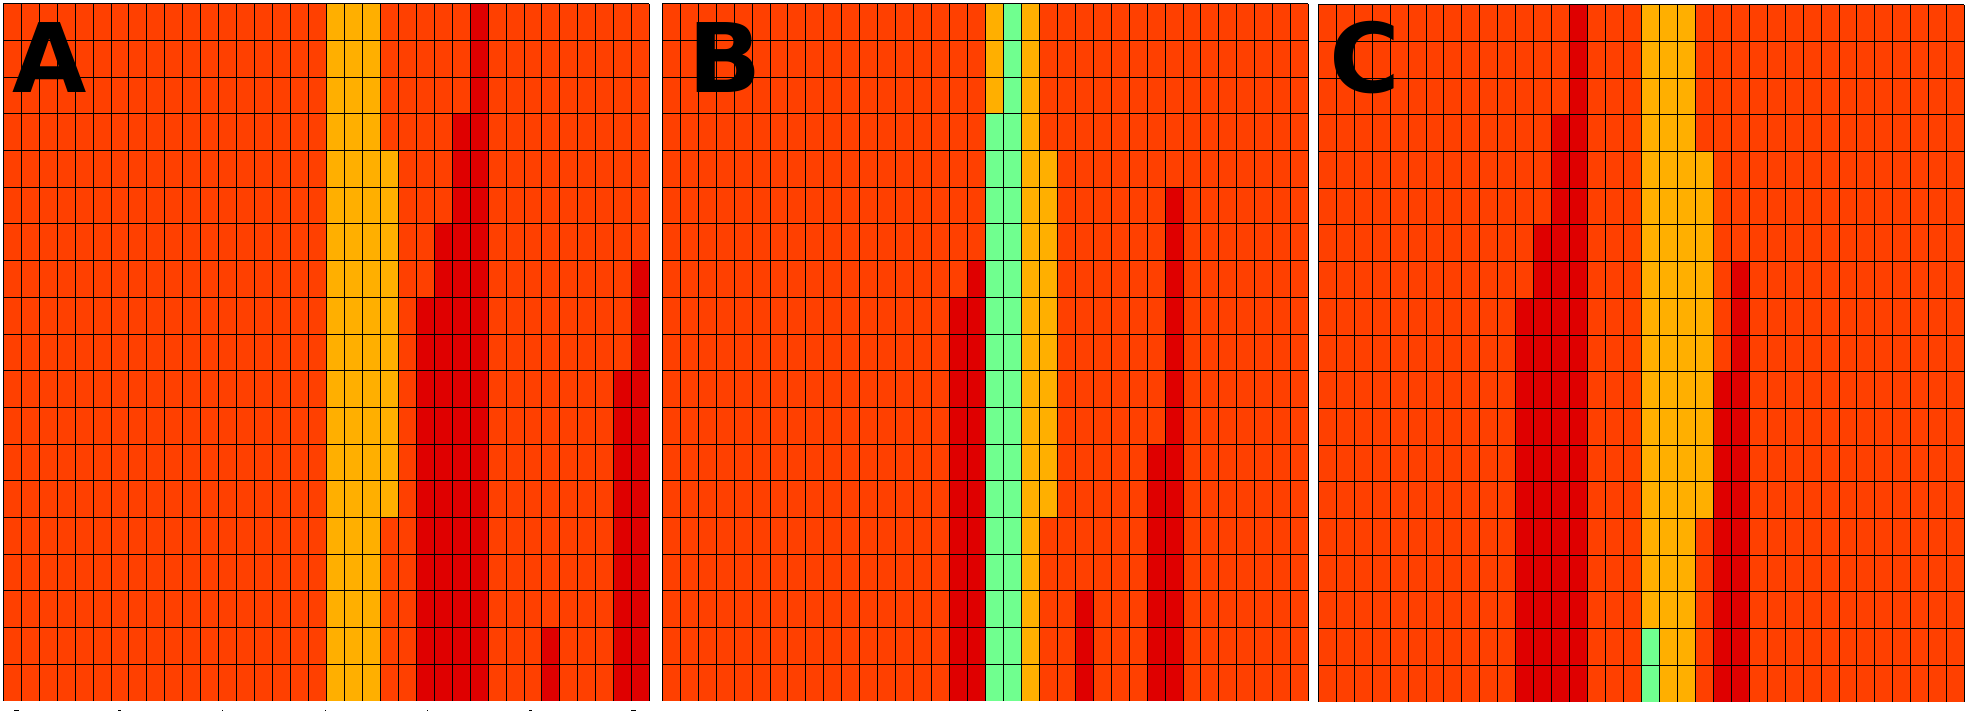
\includegraphics[width=1.0\linewidth]{./images/sequential.png} \quad 
  \end{center}
  \caption{Two superimposition of two maps on top of each other as one of the objects move}
  \label{fig:sequential}
\end{figure}



Figure 6 demonstrates the shifting of feasibility maps over each other to find proper grasps that satisfy all the tasks. 


%==================================================================================================
\begin{algorithm}[ht!]
  \SetCommentSty{emph}
  \KwIn{$\{\hat{h}, \check{h}, \hat{\theta}, \check{\theta}\}$: min/max height and angle limits, 
  $\{\delta h, \delta \theta\}$: increments, $R$: robot, $W$: world,
  \\ \hspace{3.5em}$\mathbb{T}$: object poses for tasks}
  \KwResult{$\{h,\theta\}$: grasp pose, $\delta_i$: task rotations }
  \For(\tcp*[f]{ Generate maps for each task }){$T \in \mathbb{T}$, $i \leftarrow 0$} {
    $W.setObjectPose(T)$; \\
    $M[i] = $CreateMap$(\hat{h}, \check{h}, \hat{\theta}, \check{\theta}, R, W);$\\
    $i \leftarrow i + 1$; 
  }
  
  \For(\tcp*[f]{ Iterate through object height}){$h \leftarrow \hat{h}$ \KwTo $\check{h}$} {
    $\theta^* \leftarrow -1$; \\
    \For(\tcp*[f]{ Find grasp pose on 1st object}){$\theta \leftarrow \hat{\theta}$ \KwTo $\check{\theta}$} {
      \If{$M[(h-\hat{h})/\delta h][(\theta-\hat{\theta})/\delta \theta] = 1$} {
	$\theta^* \leftarrow \theta;$ \\ 
	\textbf{break;} \\
      }
      $\theta \leftarrow \theta + \delta \theta;$ \\
    }
    \lIf{$\theta^* = -1$}
      \textbf{continue;} \\
      \BlankLine
      \BlankLine
    $foundAll \leftarrow true;$ \\
    \For(\tcp*[f]{ Find grasps for each task}){$T \in \mathbb{T}$, $i \leftarrow 0$} {
      \For{$\theta \leftarrow \hat{\theta}$ \KwTo $\check{\theta}$} {
	\If{$M[(h-\hat{h})/\delta h][(\theta-\hat{\theta})/\delta \theta] = 1$} {
	$\mathbb{\delta}_i \leftarrow \theta - \theta^*;$ \\ 
	\textbf{break;} \\
      }
      $\theta \leftarrow \theta + \delta \theta;$ \\
    }
    \If{$\mathbb{\delta}_i = \emptyset$} {
	  $foundAll \leftarrow false;$ \\	
	  \textbf{break;}\\
	}
    }
    \lIf{$foundAll$} \textbf{return} $\{h,\theta^*,\delta_i ~ \forall i\};$\\
    $h \leftarrow h + \delta h;$
  }
   
  \Return{$\emptyset$}; 
  \caption{Single Grasp for Sequential Tasks}
\end{algorithm}



%==================================================================================================
\subsection{Reasoning about Handprints for Bimanual Tasks}

Figure 7 demonstrates the projection of handprints onto the surface manifold where two hands
drawn with blue and yellow profiles can be seen colliding with each other. The algorithm 3
uses a hill-climbing approach to minimize the intersection of handprints to move the hands
further away from each other as can be seen on the right hand side of Figure 7. The computation of the hand positions were in average 23 milliseconds especially when there was a large space of feasible grasps.

\begin{algorithm}[ht!]
  \SetCommentSty{emph}
  \KwIn{$\{\hat{h}, \check{h}, \hat{\theta}, \check{\theta}\}$: min/max height and angle limits, 
  $\{\delta h, \delta \theta\}$: increments, $\mathbb{R}$: robots, $W$: world,
  \\ \hspace{3.5em} $\mathbb{H}$: hand prints}
  \KwResult{$\{h_i, \theta_i\}$: grasp poses for each robot}
  
  \For(\tcp*[f]{ Generate maps for each robot }){$R \in \mathbb{R}$, $i \leftarrow 0$} {
    $M[i] = $CreateMap$(\hat{h}, \check{h}, \hat{\theta}, \check{\theta}, R, W);$\\
    $i \leftarrow i + 1$; 
  }
  
  \For{$restart \leftarrow 0$ \KwTo MAX\_RESTARTS} {
  \BlankLine
    \For(\tcp*[f]{ Sample contacts }){robot $R \in \mathbb{R}$, $i \leftarrow 0$} {
      $[h_i, \theta_i] \leftarrow random(\hat{h}, \check{h}, \hat{\theta}, \check{\theta}, \delta h, \delta \theta);$ \\
      $i \leftarrow i + 1$;\\ 
    }
    \BlankLine
    \tcp{ Minimize collisions by moving random grasp}
    \For{$iters \leftarrow 0$ \KwTo MAX\_ITERS} {  
      
      \tcp{ Stop if all the grasps are collision free}
      \lIf{$W.collisionFree()$} \textbf{return } $\{h_i, \theta_i\}$;\\ 
      \BlankLine
      
      $R \leftarrow \mathbb{R}[random()]$;  \tcp*[f]{ Choose random robot}\\
      $dirs \leftarrow [\{\delta h,0\}, \{0, \delta \theta\}, \{-\delta h, 0\}, \{0, -\delta \theta\}]$; \\
      
      $minNumColls \leftarrow \infty, ~ bestDir \leftarrow \emptyset; $ \\
      \For{$dir \in dirs$} {
	  
	$h^* \leftarrow h_R + dir[0], ~\theta^* \leftarrow \theta_R + dir[1];$ \\
	\lIf{$M[(h^*-\hat{h})/\delta h][(\theta^*-\hat{\theta})/\delta \theta] = 0;$}
	  \textbf{continue;} 
	
	$numColls \leftarrow $countCollisions($W$); \\
	\If{$numColls < minNumColls$} {
	  $minNumColls \leftarrow numColls;$ \\
	  $bestDir \leftarrow dir;$
	}
      }
      
      \tcp{ Update grasp with minimum collision direction}
      $h^* \leftarrow h_R + dir[0], ~\theta^* \leftarrow \theta_R + dir[1];$ \\
      $h_r \leftarrow h^*, \theta_r \leftarrow \theta^*$;
      
    }
  }
  
  
  \Return{$\emptyset$}; 
  \caption{Collaborative Grasps on Single Task}
\end{algorithm}








\begin{figure}[t]
  \begin{center}
    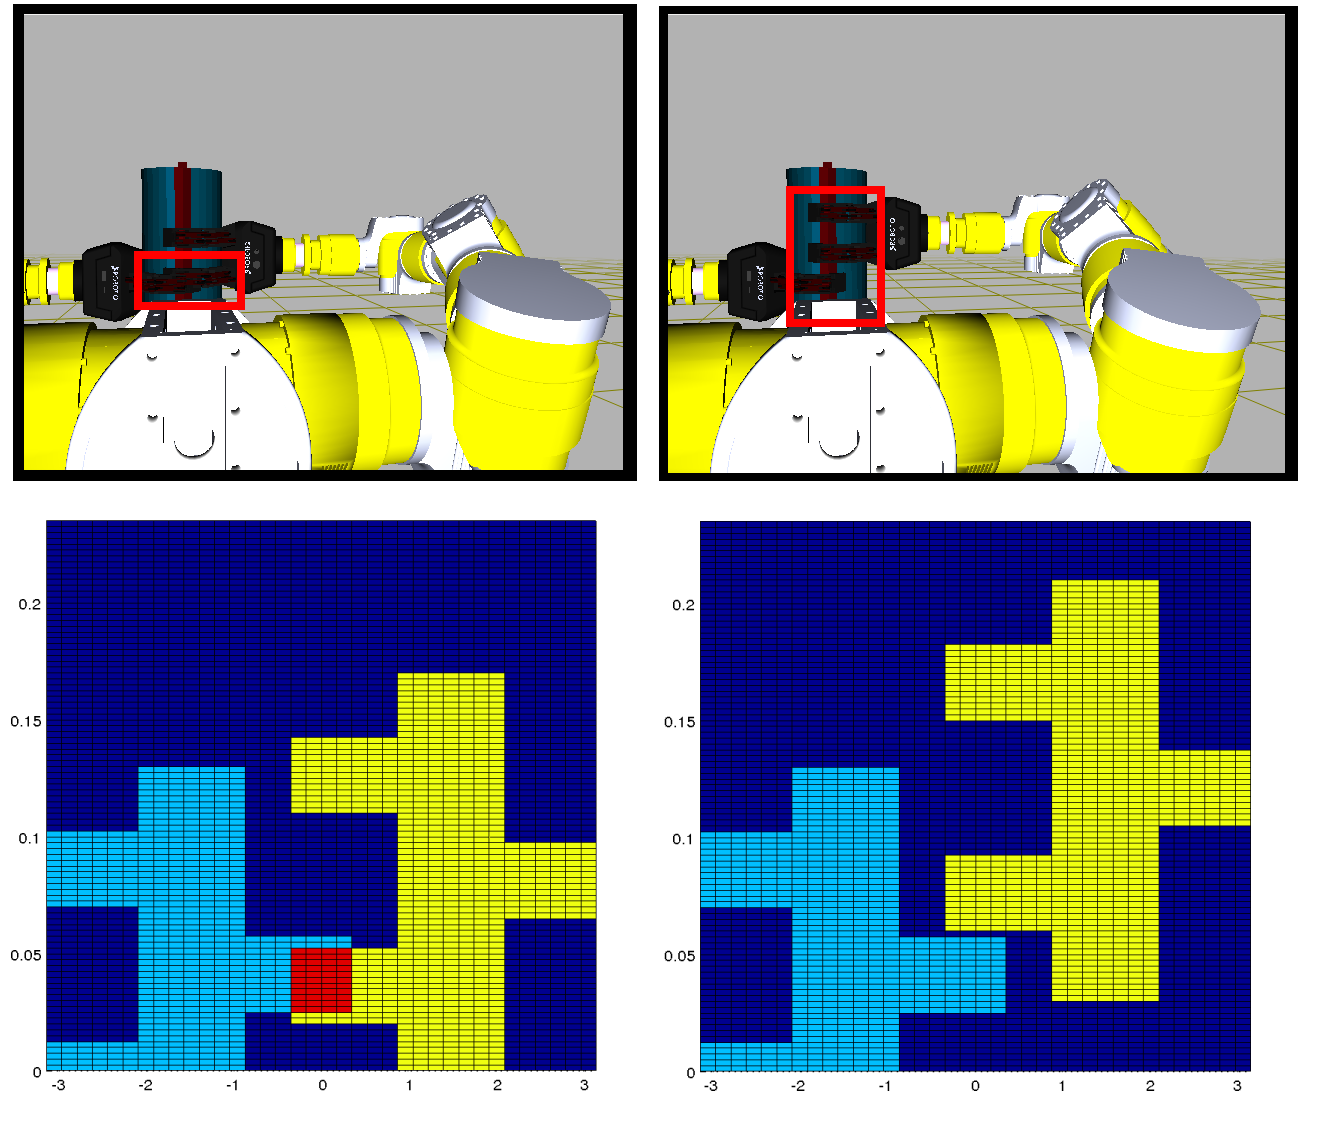
\includegraphics[width=1.0\linewidth]{./images/prints.png} \quad 
  \end{center}
  \caption{The projection of hand prints onto the object surface and the detection of finger collisions}
%   \caption{A of a
%   rotationally symmetric object. The axis $\vech{a}$ corresponds to the polar axis, while $\vech{h}$
%   is the axis of symmetry. Any point on the surface can be represented using height $h$, radius $r$,
%   and angle $\theta$. }
  \label{fig:prints}
\end{figure}


\begin{figure*}[t]
  \begin{center}
    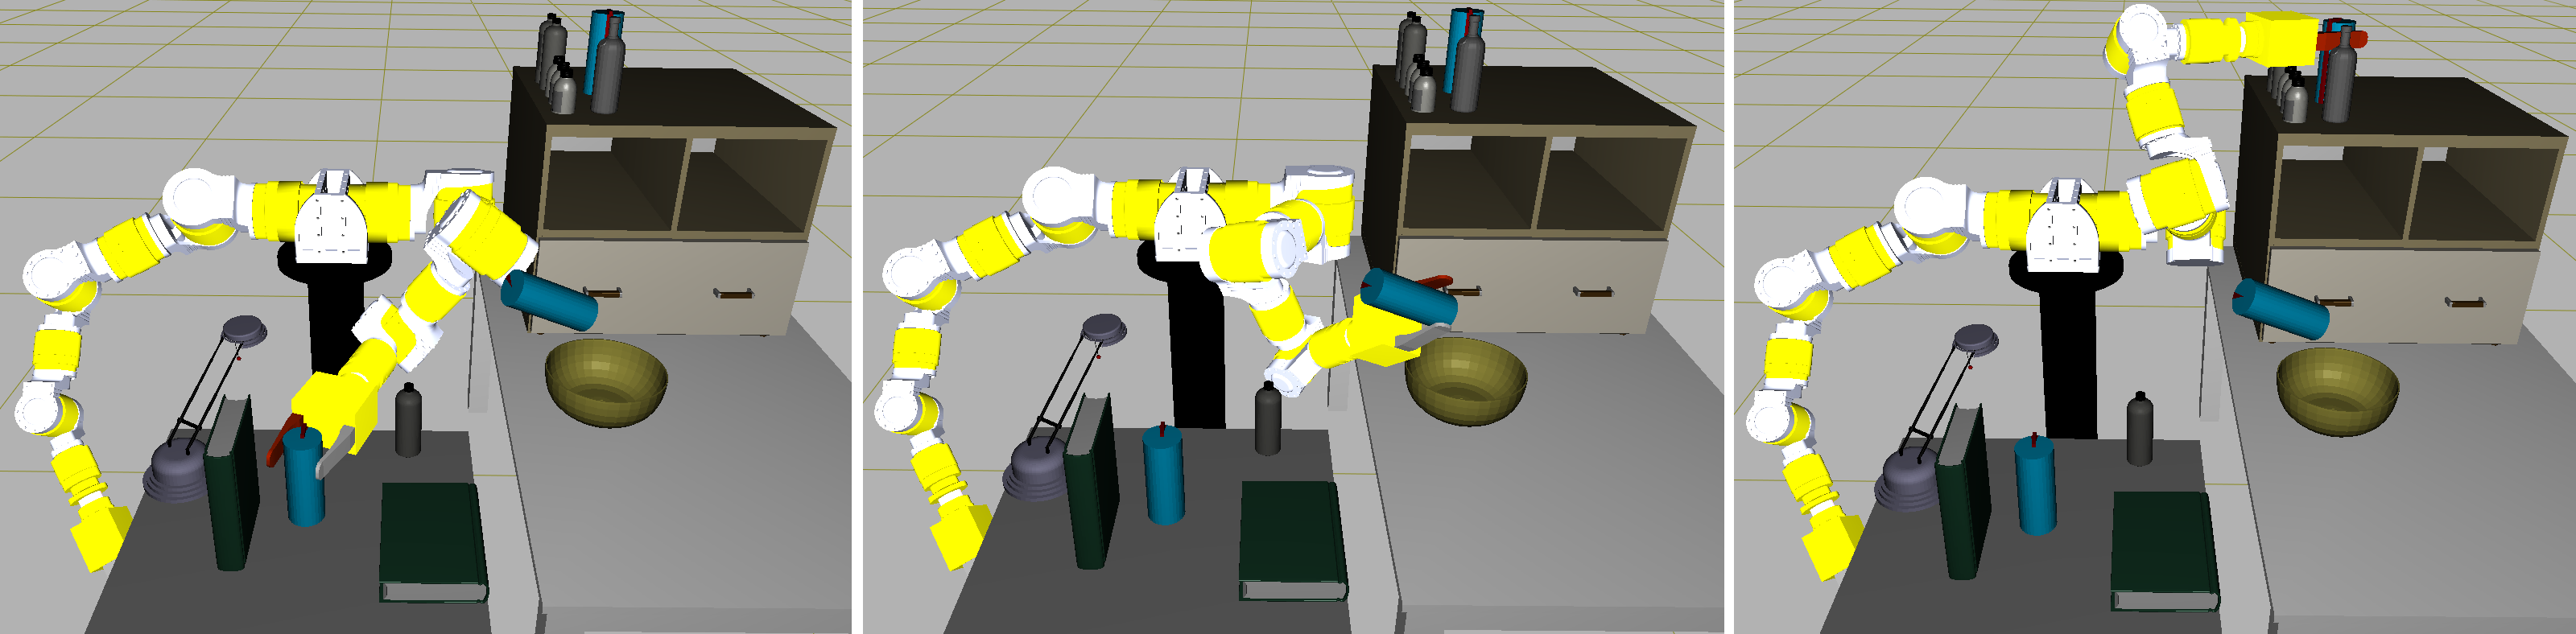
\includegraphics[width=0.85\linewidth]{./images/sequence.png} \quad 
  \end{center}
  \caption{Computation of a single grasp across multiple tasks where the robot has to pick up a bottle, pour its contents into a bowl and place it down.}
  \label{fig:sequence}
\end{figure*}















% Pic6: Rod through 3 tasks (superimposed)

% Pic7: Hand prints of two robots (two different robot hands, robotiq vs. tweezer)
% Pic8: Picture of two robots in front of each other, hand over

% offline experiment: how fast is map generation? 
% online experiment: how fast is sequence generation?
% quality? how good? alternative solutions?
% Pic8: 3D blob
% 2 different domains

\section{Discussion} 
The presented planner can be seen as a first prototype of grasp planning
algorithms that exploit symmetry and other shape properties. The main contribution
is a low-dimensional representation that allows us to store and 
analyze information about grasp feasibility for sequential or parallel 
grasping actions. While we showed that this can be used for efficient planning, there
are various aspects of our approach that need further investigation. At the moment 
we assume a discretization of the manifold. It is unclear how this discretization affects
the robot performance and how the discretization parameters need to be chosen. 
So far, we have shown that grasps can be rotated around the axis of symmetry
without modification. However, if the hand is moving up and down along the axis
of symmetry, the hand shape might have to be changed. This is particularly true in
cases where the object radius drastically changes, i.e. very curvy objects. In such 
cases, the hand shape needs to be adapted to the new radius. We believe that, similar
to the HSV color space in computer vision, we can create a 3D space which augments
the current manifold with another dimension for the radius at different heights.
This would allow us to model hand shape variations along the axis of symmetry.
So far, our study has shown that object-centered representations can be very powerful
representations for grasp planning. However, we believe that more interesting 
properties and insights about such representations can possibly be identified.
The key to grasp planning with foresight, is to use prior knowledge about 
re-occurring and natural shape properties, e.g. symmetries and extrusions, 
to generate low-dimensional grasp representations. 

\section{Conclusion}

In this paper we presented a grasp planning algorithm
that exploits rotational symmetries for generating task-constrained grasps. One of the major results is presented in Figure 8 where a sequence of tasks have been considered to compute a single grasp that satisfies all of their constraints. The algorithm is particularly suited for grasp planning with several subtasks or several interacting agents. The key insight of the paper is that re-occurring patterns in the geometry of shapes can be exploited to drastically reduce the space of solutions. To this end, we introduced a low-dimensional, object-centered representation for grasp planning which is based on rotational symmetries. Since such object are symmetric, any stable grasp can be rotated around the axis yielding a family of feasible grasps. We presented early results showing that this property allows us to generate multiple grasps around an object, which is useful for bi-manual tasks and cooperative robot hand over tasks.         
\bibliographystyle{plain}
\bibliography{draft}
\end{document}
